\documentclass[border=2mm]{standalone}
\usepackage{tikz}

%If you create a new command to draw a cube, you can use them as building blocks. 
% drawbox => a cube of unit sides
%This command takes 4 arguments: an x-coordinate, a y-coordinate , a z-coordinate of the bottom left corner and a fill-colour. ((1,1,1) being the leftmost and downmost block).
\newcommand{\drawbox}[4]{
    \pgfmathsetmacro \angle {30}
    \pgfmathsetmacro \xd {{2/3*cos(\angle)}}
    \pgfmathsetmacro \yd {{2/3*sin(\angle)}}
    \pgfmathsetmacro \x {{#1-1+(#2-1)*(\xd)}}
    \pgfmathsetmacro \y {{#3-1+(#2-1)*(\yd)}}
    % a cube = 3 faces shown, 
    \draw[thick,fill=#4] (\x,\y) -- (\x+1,\y) -- (\x+1,\y+1) -- (\x,\y+1) -- cycle;% 1st face of the cube
    \draw[thick,fill=#4] (\x,\y+1) -- (\x+\xd,\y+1+\yd) -- (\x+1+\xd,\y+1+\yd) -- (\x+1,\y+1) -- cycle; % second face (top)
    \draw[thick,fill=#4] (\x+1,\y+1) -- (\x+1+\xd,\y+1+\yd) -- (\x+1+\xd,\y+\yd) -- (\x+1,\y) -- cycle;
}


\begin{document}
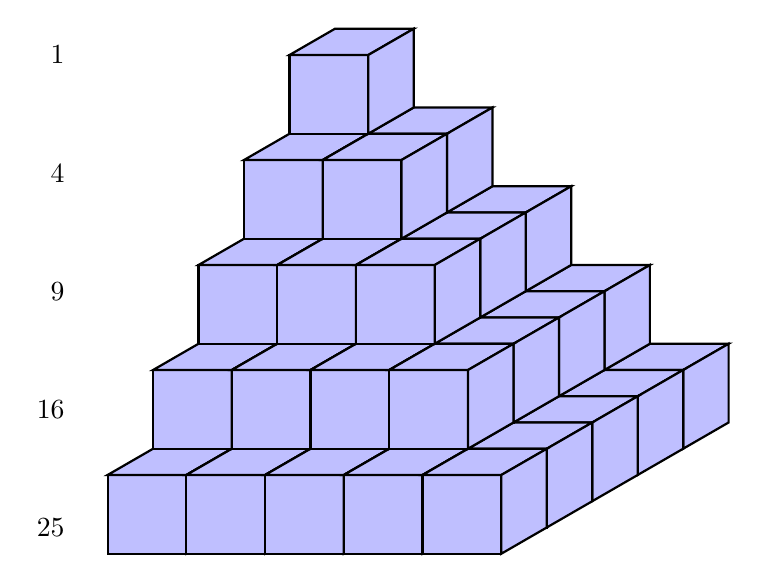
\begin{tikzpicture}
    \drawbox{4}{4}{1}{blue!25}
    \drawbox{4}{3}{1}{blue!25}
    \drawbox{4}{2}{1}{blue!25}
    \drawbox{4}{1}{1}{blue!25}


    \drawbox{0}{0}{1}{blue!25}
    \drawbox{1}{0}{1}{blue!25}
    \drawbox{2}{0}{1}{blue!25}
    \drawbox{3}{0}{1}{blue!25}
    \drawbox{4}{0}{1}{blue!25}

    % second row
    \drawbox{3}{4}{2}{blue!25}
    \drawbox{3}{3}{2}{blue!25}
    \drawbox{3}{2}{2}{blue!25}

    \drawbox{0}{1}{2}{blue!25}
    \drawbox{1}{1}{2}{blue!25}
    \drawbox{2}{1}{2}{blue!25}
    \drawbox{3}{1}{2}{blue!25}
    
    % third row
    \drawbox{2}{4}{3}{blue!25}
    \drawbox{2}{3}{3}{blue!25}

    \drawbox{0}{2}{3}{blue!25}
    \drawbox{1}{2}{3}{blue!25}
    \drawbox{2}{2}{3}{blue!25}

     % fourth row
    \drawbox{1}{4}{4}{blue!25}

    \drawbox{0}{3}{4}{blue!25}
    \drawbox{1}{3}{4}{blue!25}
    % final row
    \drawbox{0}{4}{5}{blue!25}

    \draw[] node[ left,scale=1] at ( -2,   0) {$25$};
    \draw[] node[ left,scale=1] at ( -2,   1.5) {$16$};
    \draw[] node[ left,scale=1] at ( -2,   3) {$9$};
    \draw[] node[ left,scale=1] at ( -2,   4.5) {$4$};
    \draw[] node[ left,scale=1] at ( -2,   6) {$1$};

\end{tikzpicture}



\end{document}